% ************************************************
\chapter{Network Model}\label{ch:Network Model} 
% ************************************************

Referring to anisotropic characteristics in local cortical circuits of
the rat's brain, a network model implementing anisotropic tissue
geometry is developed. The introduction of a rewiring algorithm and
qualitative anisotropy measure %quantitative ??
lay the foundation for the analysis of structural aspects of this
model in Chapter~\ref{ch:structural_aspects}.

\parskip = \baselineskip %??
\setlength{\parindent}{0pt}

%\section{Introduction}\label{sec:intro_model}

\section{Anisotropy in Neural Connectivity}\label{sec:biol_anisotropy}

% The field of neurogeometry is trying to answer the question when
% synaptic connections . Several studies
% report \parencite{Stepanyants2005}
% Axonal and synaptic is uncorrelated \parencite{Stepanyants2005} 

% The main stem of a pyramidal cell's axon , laying the foundation for
% anisotropy in connectivity.



% Research in the field of neurogeometry yields a simple rule for
% networks to be connected 

% Thus axon morphology distinctively determines network 
% connectivity. \marginpar{axon
% morphology determines connectivity}

Neurogeometry\index{neuro geometry} addresses the problem of inferring
synaptic connectivity from the geometric shapes of axon and
dendrites. A fundamental concept in this field is that of
\textit{potential synapse}\index{potential synapse}
\parencite{Stepanyants2002}. Defined as the potential axonal-dendritic
connection of two neurons, present whenever the axon of one neuron is
within a spatial distance $s$ of the dendrite of the other, it is a
necessary, although not sufficient, condition for the formation of a
synaptic connection (\autoref{fig:potential_synapse}). The existence of such close
appositions strongly depends on dendritic and axonal anatomy;
identification of defining morphological characteristics in both axon
and dendrites would therefore allow for an abstracted model of network
connectivity. It is the hope that such a model, motivated from the
geometry of the cortical neuron's functional compartments, yields interesting
connectivity and dynamics.

% \vspace{0.5cm}
% \begin{figure}[!htbp] 
%   \centering 
%   \includegraphics[width=0.55\textwidth]{%
%     gfx/img/potential_synapse1.png}%
%   \caption{\textbf{Tracing axonal branching of a pyramidal cell}.}%?? not the right caption    
%   \label{fig:potential_synapse}
% \end{figure}

\vspace{0.5cm}
\begin{figure}[!htbp]
\captionsetup{format=plain}
\floatbox[{\capbeside\thisfloatsetup{capbesideposition={right,top},capbesidewidth=0.45\textwidth}}]{figure}[\FBwidth]
{\includegraphics[width=0.45\textwidth]{gfx/img/potential_synapse1.png}}
{\caption{\textbf{Potential Synapse}  \textbf{a)} 3-D reconstruction
    showing dendrite of pyramidal cell in red, axon of 
    cell in red. Image from \textcite{Stepanyants2005}.}\label{fig:potential_synapse}}
\end{figure}
\vspace{0.3cm}

Finding such defining characteristics however is difficult, as axonal morphology is,
in general, highly diverse.
\parencite{Debanne2004}. Across different species,
%------------------------------------------------
\marginpar{high variability in axonal morphology} 
%------------------------------------------------ 
distinct regions in the central nervous system and different neuron
types, axons display a wide variety of shapes characterized by
morphometric parameters such as total length, branching complexity and
axonal extent \parencite{Ropireddy2011}. Typical examples of distinct
morphology include the T-shaped axons of cerebellar granule cells
branching only at a singular point, and axons of hippocampal CA3
pyramidal cells, which, in stark contrast, have at least 100 to 200
branch points and a total axon length between 150 and
\SI{300}{\milli\meter}. %??citations from Debanne?

It is therefore imperative to confine this analysis to a specific
brain region and neuron type. In this study, we set the focus on
circuits of pyramidal cells in the mammalian cortex. Being among the
most well studied local networks, the . Even more specifically, local
circuits of thick tufted layer V pyramidal neurons in the rat's
somatsosensory cortex will serve as a benchmark f


Axons of pyramidal cells in the mammalian cortex are well
described. From the soma the single main stem of the axon
originates and then projects downwards, describing a trajectory resembling
a straight line \parencite[p.~67]{Braitenberg_Cortex}. Within a
distance of 300-\SI{500}{\micro\meter}, the axon arborizes building
as many as 2nd and 3rd order collateral branches. Again
constituting a complex tree-like structure. 

Experiments are constrained by a typical slice thickness of
\SI{300}{\micro\meter}. On this scale, 3-D reconstruction from labeled
thick tufted layer V pyramidal cells illustrates characteristic
morphology of the axonal tree (\autoref{fig:romand_axon_trace}). Downwards, branching,
vertically. 


, showing an apparent anisotropy in neural connectivity, aligning with
the growth direction of axon's main stem (\autoref{fig:axon_heat}).



Using image manipulation software to trace axonal trees in a
sample of five reconstructions of TTL5 neurons,   
 
In a sample of 5 reconstructions, the respective axonal
trees where traced using image manipulation o 


Downwards, branching,
vertically. Tracing the axon with a image manipulation program, we
obtain a heat map (\autoref{fig:axon_heat}).

Dendritic morphology in layer V is also well
described. \marginpar{dendritic morphology in layer V} Bipartite,
neglect apical dendrite.


Combing the heatmaps, we obtain clear evidence for anisotropy. 




% Thick tufted pyramidal cells in the rat's somatosensory cortex 

% Owing to this diversity, it is impossible to and it
% is our intent to focus on a specific neuron type and brain region.

% Neuron morphology as well as network connectivity in the rat's
% somatosensory cortex has been thoroughly studied. Even more
% specifically, thick tufted layer V have been the target of studies. 
% \marginpar{focus on TTL5 neurons}




% %?? Neuromorpho evidence 


% Neuron morphology and connectivity in the rat's somatosensory cortex
% has been thoroughly studied. As s. 



% Identifying anisotropy in neural connectivity as an interesting . In
% this thesis 
% In this study is more specifically focusing in pyramidal neurons in 


\vspace{0.5cm}
\begin{figure}[h] 
  \centering 
  \makebox[0.875\textwidth]{%
    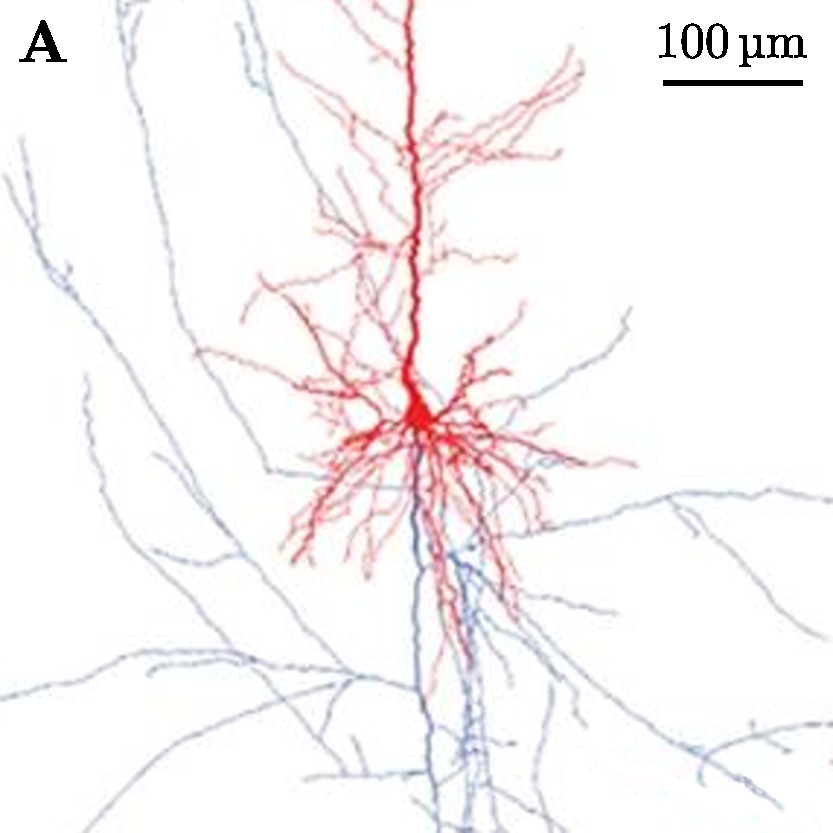
\includegraphics[width=0.4\textwidth]{%
      gfx/img/network_model/p14rr_1_traced_soma_unit_A.pdf}%
    \hfill
    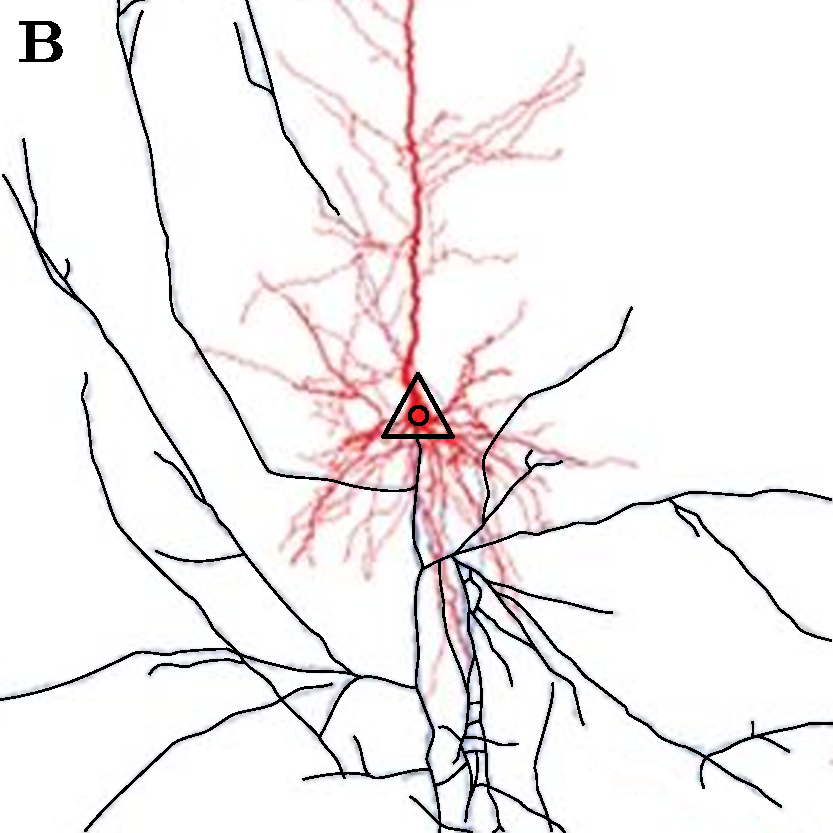
\includegraphics[width=0.4\textwidth]{%
      gfx/img/network_model/p14rr_1_traced_soma_unit_B.pdf}% 
    }%

  \caption{\textbf{Tracing axonal branching of a pyramidal cell} 
    In a 3-D model reconstructed from biocytin-labeled thick-tufted
    layer V pyramidal cells in the somatosensory cortex of  postnatal
    (day 14) Wistar
    rats, \textcite{Romand2011} depict dendritic compartments in
    red, axonal compartments in blue. 
    \textbf{A)} A \SI{600}{\micro\meter} window centered on the
    soma of the pyramidal cell shows the main stem of the cell's axon projecting downwards in
    a straight line, collaterals branching at various angles. \textbf{B)} Using
    image manipulation software, axon morphology was manually traced
    and is emphasized in black.}%?? this doesn't hit anisotropy idea yet
    
  \label{fig:romand_axon_trace}
\end{figure}






\vspace{0.5cm}
\begin{figure}[h] 
  \centering 
  \makebox[0.875\textwidth]{%
    \begin{overpic}[width=0.4\textwidth]{gfx/img/network_model/p14rr_1_trace_soma.pdf}
      \put(3,92){\small\textbf{A}}
    \end{overpic}
    \hfill
    \begin{overpic}[width=0.4\textwidth]{gfx/img/network_model/axon_heat_correct_soma.png}
      \put(3,92){\small\textbf{\textcolor{white}{B}}}
    \end{overpic}
    }%
    \caption{\textbf{Overlay of 5 axonal branches} \textbf{A)} Axon
      collaterals of a single pyramidal cell as extracted in
      \autoref{fig:romand_axon_trace}. \textbf{B)} Consecutively
      overlaying extracted axon trees from five different neurons from
    \textcite{Romand2011} yields a dense pattern of axonal
    morphology. Heatmap shows density and illustrates the anisotropy
    in neural connectivity}%??
  \label{fig:axon_heat}
\end{figure}


\vspace{0.5cm}
\begin{figure}[!htbp]
  \makebox[0.875\textwidth]{%
    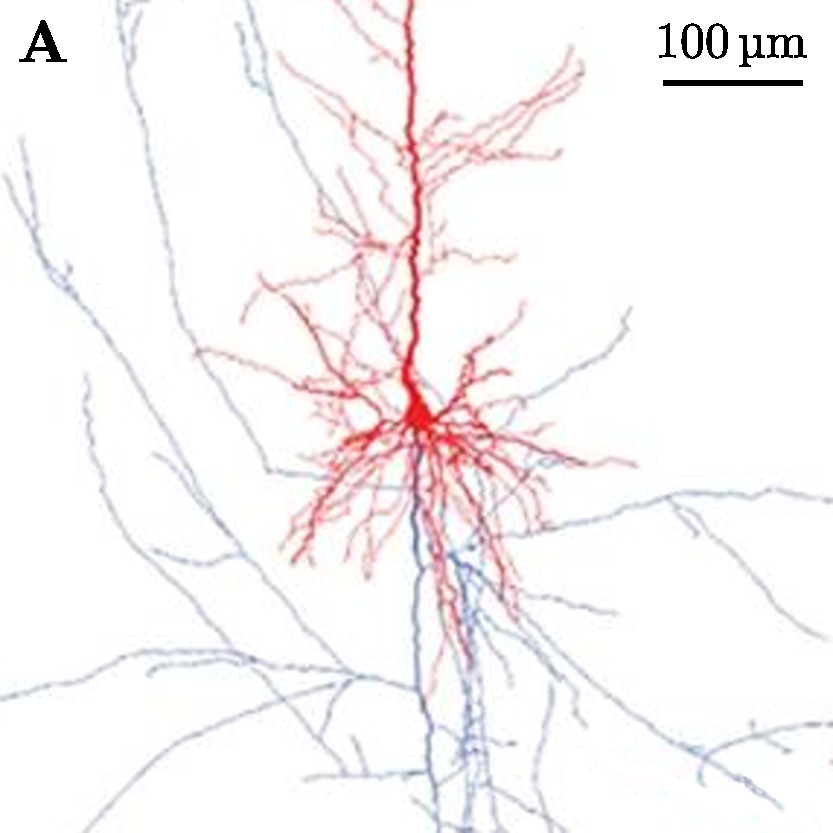
\includegraphics[width=0.4\textwidth]{%
      gfx/img/network_model/p14rr_1_traced_soma_unit_A.pdf}%
    \hfill
    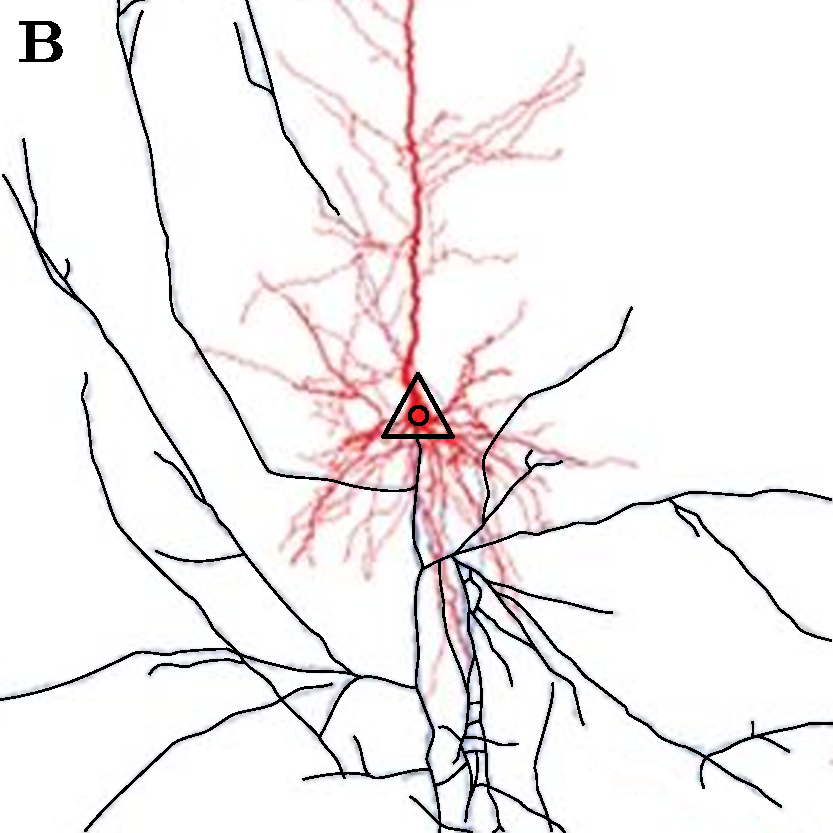
\includegraphics[width=0.4\textwidth]{%
      gfx/img/network_model/p14rr_1_traced_soma_unit_B.pdf}% 
    }%
  \vspace{0.3cm}
  \makebox[0.875\textwidth]{%
    \begin{overpic}[width=0.4\textwidth]{gfx/img/network_model/p14rr_1_dendrite_trace_scale.pdf}
      \put(3,92){\small\textbf{C}}
    \end{overpic}
    \hfill
    \begin{overpic}[width=0.4\textwidth]{gfx/img/network_model/dendrite_heat_correct_soma.png}
      \put(3,92){\small\textbf{\textcolor{white}{D}}}
    \end{overpic}
    }%
  \caption{\textbf{Overlay of 5 axonal branches} \textbf{A)} Axon
      collaterals of a single pyramidal cell as extracted in
      Figure~\ref{fig:romand_traced}. \textbf{B)} Consecutively
      overlaying extracted axon trees from five different neurons from
      \textcite{Romand2011} yields a dense pattern of axonal
      morphology. Heatmap shows density and illustrates the anisotropy
      in neural connectivity}%?? caption wrong
  \label{fig:dendrite_heat}
\end{figure}






\clearpage
\section{Anisotropic geometric graph model}\label{sec:network_model}

Model tries to be geometric and simple. We therefore

Along the main stem of the axon in constant width. \marginpar{Variable
  width later!}%?? When?

\newpage
\section{Distance dependent connectivity}\label{sec:dist_depend_con}

In Gilbert's random graph model $G(n,p)$, 
\marginpar{Random Graph  Model section~\ref{sec:gilbert_graph}} %?? TITLE
probability of connection $p$ is independently chosen and a fixed
value for all vertex pairs. The anisotropic geometric graph model
introduced in the last %(true??)
section is itself a random graph model - node positions as well as
preferred directions of connection are randomly, uniformly
distributed. In contrast to Gilbert's model however, neither is the
probability of connection between a given vertex pair independent of
the realization of other edges in the graph, nor is it a fixed value -
probabilities strongly depend on internode distance in the
anisotropic geometric graph model introduced.

Analyzing dependencies in the anisotropic model, specifically by
identifying prevalent patterns of connectivity and relating these
modes of non-randomness to biological findings, is the main focus of
Chapter~\ref{ch:structural_aspects}. However, such structural
correlations may not necessarily be an inherent feature of the
network's anisotropy - distance dependent connectivity alone, as
imposed by the model's specific geometry, may be the cause for
emerging dependencies. It is therefore a crucial initial task to map
the anisotropic model's distance dependent connection
probability. Inferring connection probability as a function of
internode distance and comparing it with computational results, in
this section we explore distance connectivity of the anisotropic
network model, securing a vital component in the analysis of
structural features.

Consider a graph $G$. In Gilbert's random graph model the probability
$p$ for a edge between nodes $v,w \in V(G)$ to be realized is a fixed
value; in a geometric graph it is more generally a function of the
distance between the nodes, $d(v,w)$. In short, we write $p(x)$ to
denote the probability that a vertex pair of distance $x$ is
connected,

\[p(x) := P\left[(v,w)|\,d(v,w)=x\right].\]
Owning to the abstract geometric model we defined, this connection
probability is easily computed.

\begin{proposition} %?? make proposition or something
In the anisotropic geometric graph model distance depend connection
probabilities are computed as 
\[
p(x) = \begin{cases} 0.5 & \mathrm{for} \,\, x\le w/2 \\
                       \frac{1}{\pi}
                       \operatorname{arcsin}(\frac{x}{2w}) &
                       \mathrm{for} \,\, x >
                       w/2. \end{cases}
\]
\end{proposition} 

\begin{proof}
  To see this, consider a given source vertex $v$ at $(0,0)$ and a
  possible target $w$, such that $d(v,w) = x$. We may then express the
  target coordinates as $x e^{i\varphi}$, $0 \le \varphi < 2\pi$.

  Figure~\ref{fig:geomtr_prb} illustrates for which angles
  $\varphi$ the node $w$ becomes a valid target for an edge from
  $v$. This intervall

  \begin{figure}[h] 
    \centering 
    \makebox[0.85\textwidth]{%
      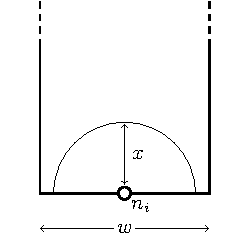
\includegraphics[width=0.4\textwidth]{gfx/tikz/geomtr_prb_05.pdf}%
      \hfill
      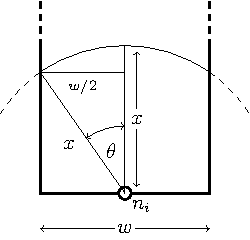
\includegraphics[width=0.4\textwidth]{gfx/tikz/geomtr_prb.pdf}% 
    }%
    %\caption{}%??
    \label{fig:geomtr_prb}
  \end{figure}

  For a general $v$ make coordinate transformation

\end{proof}

We can verify this result by computationally extracting the distance
dependencies in the sample graphs generated. 

\begin{figure}[h]
  \centering
  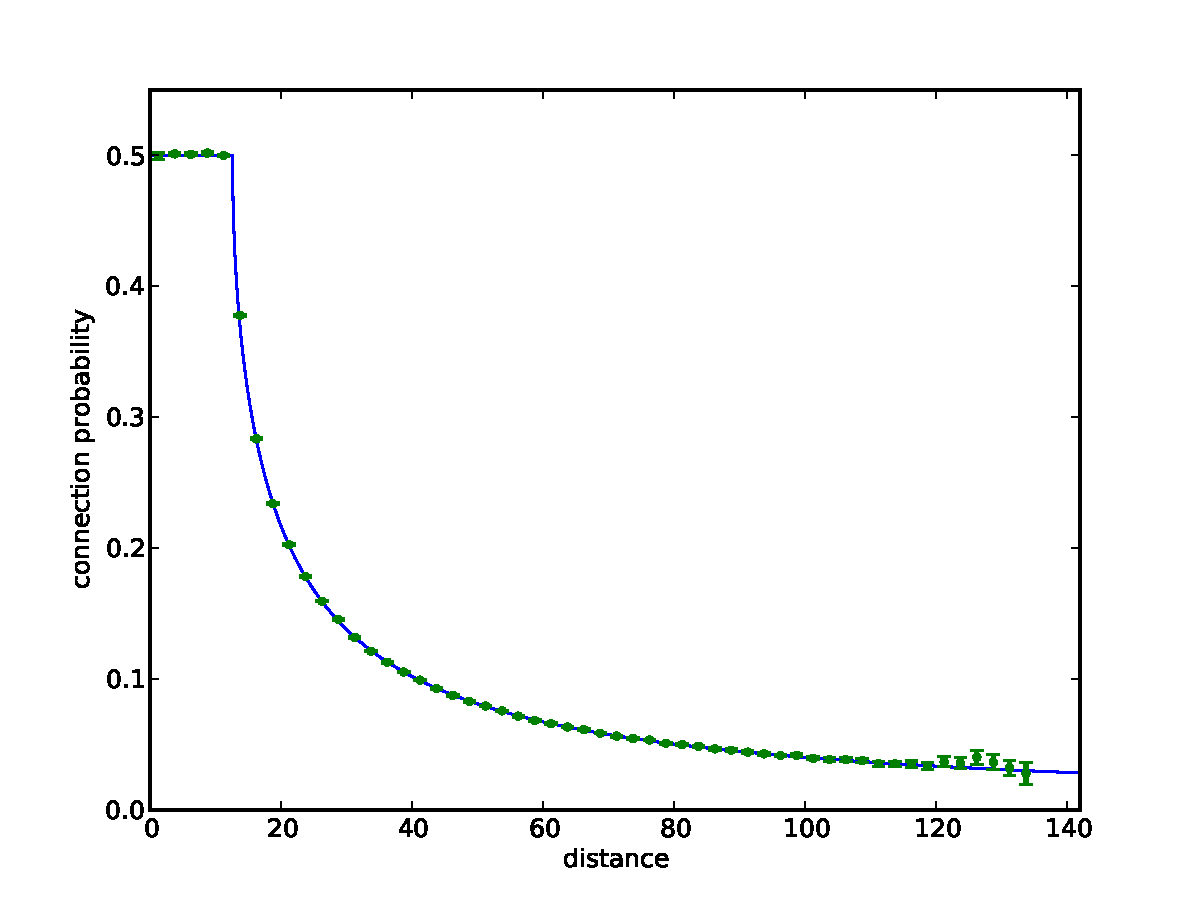
\includegraphics[width=0.7\linewidth]{gfx/plots/test.pdf}
  \caption{\textbf{Distance dependent connection probabilities}}%??
  \label{fig:something_else}%??
\end{figure}





\section{Rewiring Methods}

In the network configuration introduced in
section~\ref{sec:network_model} strong directional anisotropy is
present: Edges originating from one node \enquote{point in the same
  direction}, that is they connect to other nodes which cluster around
a. In this section we introduce an algorithm

\vspace{0.5cm}
\begin{figure}[h] 
  \centering 
  \makebox[0.85\textwidth]{%
    %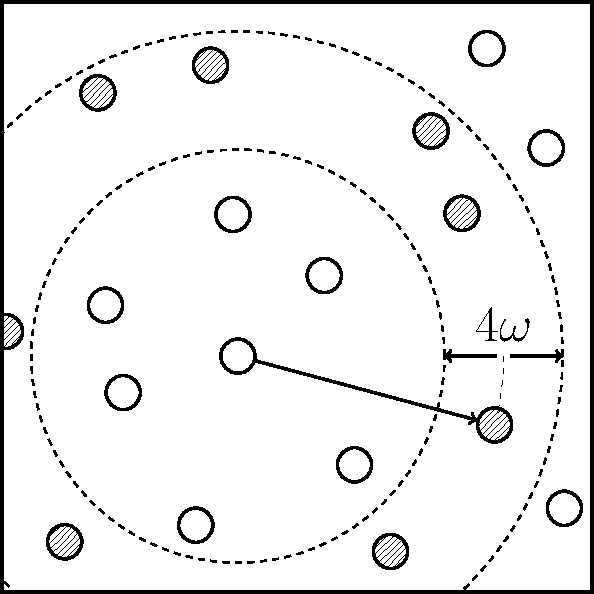
\includegraphics[width=0.4\textwidth]{gfx/dist_rew_org.pdf}%
    \begin{overpic}[width=0.4\textwidth]{gfx/tikz/distance_rewiring.pdf}
      \put(3,105){\small\textbf{Before}}
    \end{overpic}
    \hfill
    \begin{overpic}[width=0.4\textwidth]{gfx/tikz/distance_rewiring.pdf}
      \put(3,105){\small\textbf{After}}
    \end{overpic} 
  }%
  \caption{\textbf{Rewiring}}%??
  \label{fig:distance_rewiring}
\end{figure}

 

\section{Anisotropy Measure}


\section{Summary and Discussion}













%%% Local Variables: 
%%% mode: latex
%%% TeX-master: "../ClassicThesis"
%%% End: 
